\documentclass[letter,openridht,12pt,spanish]{report}
%Gummi|065|=)
\title{\textbf{Simulaci\'on de cinem\'atica directa de manipuladores seriales}}
\author{Cinematica\\
		Alcala Villagomez Mario\\
		Becerra I\~niguez Diego Armando\\
		Martinez Velazquez Lisbeth\\
		Murgu\'ia Ch\'avez Nadia Sarahi\\
		Ramos Ch\'avez Brian Oswaldo\\
		Ing. Mecatr\'onica 7A}
\date{27 de septiembre 2019}
\usepackage{graphicx}
\begin{document}

\maketitle

\section{Descripci\'on del movimiento}

DISMEDIC tienen una secuencia de movimientos de acuerdo a las coordenadas establecidas para el abastecimiento de medicamentos dentro de las farmacias. Con el cual se busca reducir el tiempo y el mejoramiento de la atenci\'on al cliente al momento de de surtir su receta.\\
La secuencia de movimientos consta de movimientos verticales y horientales dentro del eje "x" e "y".\\
Es decir que las barras paralelas se mueven de izquierda a derecha y viceversa de manera paralela para posicionarse en el espacio solicitado donde se encuentra el medicamento.\\
En la parte del actuador o surtidor de medicamentos cuenta con dos barras horizontales las cuales se moveran de arriba a bajo y viceverza para tomar tomar el medicamento.\\

\section{Boceto}

\begin{figure}[htp]
\centering
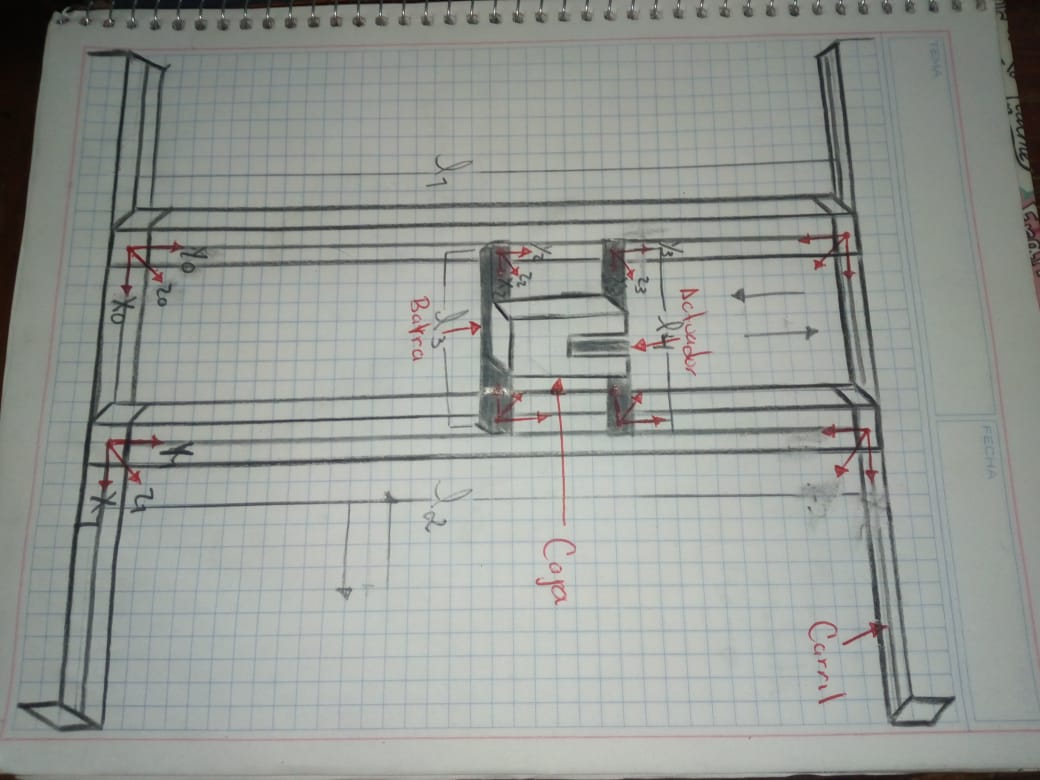
\includegraphics[width=10cm]{/home/sarha13/Escritorio/Boceto.jpeg}
\caption{Boceto}
\label{Figura 1.}
\end{figure}

\section{Tabla de movimiento de robot.}

\begin{center}
\begin{tabular}{|c|c|c|c|c|}
\hline
	Eje & $\theta_i$ & $d_{i-1}$ & $\alpha_{i-1}$ & $a_i$\\
\hline
	1 & $\theta$ & $\theta$ & $\theta$ & $l_1$\\
\hline
	2 & $\theta$ & $\theta$ & $\theta$ & $l_2$\\
\hline
	3 & $\theta$ & $d_5$ & $\theta$ & $l_3$\\
\hline
	4 & $\theta$ & $d_6$ & $\theta$ & $l_4$\\
\hline
\end{tabular}
\end{center}

El aporte en la siguiente practica se dio a cabo sobre el análisis de la movilidad y las direcciones en las que se maneja el robot cartesiano.\\
Una de sus complicaciones fue el análisis en la tabla al completar los ejes en el que se maneja, ya que tiene cierta confusión, pero se pudo completar su análisis por parte de todos los compañeros.
\section{Concluciones}

\textbf{Mario Alcala Villagomez}\\
En conclusi\'on esta pr\'actica que se desarroll\'o No fue tan complicada ya que lo único que se analiz\'o fue los movimientos del robot cartesiano con el metodo de convencion de denavit hartenberg.\\
Al igual la funci\'on que tiene este robot en la medicina y como se desarrolla para una mejoria y comodidad en el area farmac\'eutica y el mejor manejo de los medicamentos.\\
\textbf{Diego Armando Becerra I\~niguez}\\
El robot cartesiano tienen distintos usos en este caso la medicina ya que en las farmacias a\'un sigue la intervenci\'on humana y por ende hay gasto tiempo, además tendr\'ia una base de datos con la existencia de todos los medicamentos del establecimiento restando as\'i tiempo de b\'usqueda.\\
\textbf{Lisbeth Martinez Velazquez}\\
El aporte en la siguiente practica se dio a cabo sobre el análisis de la movilidad y las direcciones en las que se maneja el robot cartesiano.\\
Una de sus complicaciones fue el análisis en la tabla al completar los ejes en el que se maneja, ya que tiene cierta confusión, pero se pudo completar su análisis por parte de todos los compañeros.\\
\textbf{Nadia Sarahi Murgu\'ia Ch\'avez}\\
El an\'alisis de movimiento se realizo mediante la vizualizaci\'on de los eslabones que llevaran acabo la movilizaci\'on del robot de acuerdo a los ejes que se moveran.\\
\textbf{Brain Oswaldo Ramos Ch\'avez}\\
En el reporte de la pr\'actica se estuvo analizando sobre los desplazamientos del robot cartesiano ya que lo que hace funcional al sistema y que tiene su función de un dispersor de medicamento tanto en las coordenadas cartesianas y con el actuador central dando como funci\'on una rampa con accionamiento mecanico para que el medicamento sea transportado a la banda para que este llege a las personas que sean atendidas por los médicos dentro del establecimiento.\\
\end{document}
